\documentclass{report}
\usepackage{mathtools}
\usepackage{etoolbox}
\usepackage{amsmath}
\usepackage{siunitx}
\usepackage{tikz}
\usetikzlibrary{datavisualization}
\usetikzlibrary{datavisualization.formats.functions}
\usepackage{titlesec}[rubberchapters]
\usepackage{enumitem}
\usepackage{pgfplots}
\makeatletter
\patchcmd{\chapter}{\clearpage}{}{}{}
\makeatother
\everymath{\displaystyle}
\titleformat{\chapter}[display]
    {\normalfont\huge\bfseries}{}{0pt}{\huge}
\titlespacing*{\chapter}{0pt}{0pt}{20pt}
\pgfplotsset{width=10cm,compat=1.9}
\begin{document}
\begin{titlepage}
    \centering
    203-NYB-05\\
    Electricity and Magnetism\\
    Professor: Ernest Dubeau\par
    \vspace{5cm}
    \Large AC Circuits: Lab 1\par
    \normalsize
    By:\\
    Philipe Goulet\\
    \vspace*{\fill}
    {\today}\\
    Departement of Physics\\
    Champlain Regional College\\
    Lennoxville, Quebec, Canada
\end{titlepage}
\chapter{Prelab}

\section{An Oscilloscope is connected across a power source and the screen displays the image seen in figure. }

\subsection*{a) What is the peak voltage of the signal (include the uncertainty)?}
    \begin{gather}
        (20.0\pm0.5)\si{\volt}
    \end{gather}

\subsection*{b) What is the period of the signal (include the ucnertainty)?}
    \begin{gather}
        (0.100\pm0.005)\si{\second}
    \end{gather}

\subsection*{c) What is the frequency of the power source (include the uncertainty)?}
    \begin{align}
        f&=\frac{1}{T}\nonumber\\
         &=\frac{1}{(0.100\pm0.005)\si{\second}}\nonumber\\
         &=(10.0\pm0.5)\si{\hertz}
    \end{align}

\subsection*{d) If a DMM were to be connected across the same power source, what reading would you expect (Include the uncertainty)?}
    \begin{align}
    \Delta\si{\volt}_{rms}&=\frac{\Delta\si{\volt}_{\max}}{\sqrt{2}} \nonumber\\
                          &=\frac{(20.0\pm0.5)\si{\volt}}{\sqrt{2}}\nonumber\\
                          &=(14.1\pm0.7)\si{\volt}
    \end{align}

\subsection*{e) Write the sinusoidal function that represents the signal given off by the power source ( do not include the uncertainty)?}
    \begin{align}
        \sin(\omega t + \phi)&=\sin(2\pi f*t + \phi)\nonumber\\
        &=\sin(2\pi 10* + 0)\nonumber\\
        &=\sin(20\pi t)
    \end{align}

\subsection*{f) This power source is now connected to a single resistor with resistance $R = ( 100\pm2 )\si{\ohm}$.What is the value of $I_{\max}$ (include uncertainties)?}
    \begin{align}
        \Delta\si{\volt}_{\max}&=I_{\max}R\nonumber\\
        I_{\max}&=\frac{\Delta\si{\volt}_{\max}}{R}\nonumber\\
        I_{\max}&=\frac{(20.0\pm0.5)\si{\volt}}{(100\pm2)\si{\ohm}}\nonumber\\
        I_{\max}&=(200\pm9)\si{\milli\ampere}
    \end{align}

\subsection*{g) How much current passes through this resistor at $t = 0.0050\si{\second}$ (no uncertainties) }
    \begin{align}
        I(t)&=\frac{\Delta\si{\volt}(t)}{R}\nonumber\\
        I(0.050)&=\frac{\Delta\si{\volt}(0.050)}{R}\nonumber\\
        &=\frac{0\si{\volt}}{100\si{\ohm}}\nonumber\\
        &=0
    \end{align}

\subsection*{h) How much power ( on average ) is delivered to this resistor ( include uncertainties )?}
    \begin{align}
        P_{rms}&=\Delta\si{\volt}_{rms}I_{rms}\nonumber\\
               &=\frac{\Delta\si{\volt}_{\max}}{\sqrt{2}}\frac{I_{\max}}{\sqrt{2}}\nonumber\\
               &=\frac{(20.0\pm0.5)\si{\volt}}{\sqrt{2}}\frac{(200\pm9)\si{\milli\ampere}}{\sqrt{2}}\nonumber\\
               &=(3.17\pm0.38)\si{\watt}
    \end{align}

\subsection*{i) How much current passes through this resistor at $t = 0.025\si{\second}$ (no uncertainties) }
    \begin{align}
        I(t)&=\frac{\Delta\si{\volt}(t)}{R}\nonumber\\
        I(0.025)&=\frac{\Delta\si{\volt}(0.025)}{R}\nonumber\\
        &=\frac{20\si{\volt}}{100\si{\ohm}}\nonumber\\
        &=0.2\si{\ampere}
    \end{align}

\subsection*{j) How much current passes through this resistor at $t = 0.10\si{\second}$ (no uncertainties) }
    \begin{align}
        I(t)&=\frac{\Delta\si{\volt}(t)}{R}\nonumber\\
        I(0.10)&=\frac{\Delta\si{\volt}(0.10)}{R}\nonumber\\
        &=\frac{0\si{\volt}}{100\si{\ohm}}\nonumber\\
        &=0
    \end{align}

\chapter{Aims}

This lab was conceived to explore the basic concepts of AC circuits and observe and measure the properties of different components ( such as resistors, capacitors and inductors ) when exposed to alternating currents of various frequencies. 

\chapter{Aparatus}
\begin{itemize}[label=\textbullet]
\item Oscilloscope
    \item Stopwatch
    \item Pasco Digital Function Generator (ac source)
    \item Digital Multimeter  (\textit{BK} and \textit{Brunelle}) 
    \item Lamp
    \item A 1\si{\micro\farad} capacitor
\end{itemize}

\chapter{ AC circuit with a single resistor}

\section{Procedure}
\begin{itemize}[label=\textbullet]
    \item Replicate the circuit shown in figure 11.
    \item Turn on both digital multimeters and set them to ac mode.
    \item Set the frequency of the AC source to 1000hz.
    \item Connect the lamp to the channel A of your oscilloscope using the coaxial cable. You should observe a sinusoidal pattern on the oscilloscope’s screen.
    \item Adjust the amplitude of the AC source to have a $\Delta\si{\volt}_{\max}$ of 4.0$\si{\volt}$ as measured on the oscilloscope.  Use this value of $\Delta\si{\volt}_{\max}$ to calculate $\Delta\si{\volt}_{rms}$. Include the uncertainties.
    \item Draw a sketch of the oscilloscope screen and make sure to include a scale (and units).
    \item Use the Brunelle DMM to measure the \textit{rms} voltage across the resistor (a lamp) and use the BK digital multimeter to measure the \textit{rms} current (note uncertainties in both cases).
    \item Compare the $\Delta\si{\volt}_{rms}$  measured with the digital multimeter to the $\Delta\si{\volt}_{rms}$  calculated previously to verify whether or not the digital multimeter actually measures the \textit{rms} voltage. Make sure to account for uncertainties.
    \item Use the AC readings of both digital multimeters and Ohm’s law in AC (see theory) to calculate the resistance of the lamp (include uncertainties). Use the measure values of $\Delta\si{\volt}$ and I$_{rms}$ to determine the average power delivered to R (include uncertainties)
    \item Measure the period T of the signal on the oscilloscope’s screen. Use this measured value to calculate the frequency and compare it to the frequency given by the AC power source. (include uncertainties).
    \item Change the frequency of the AC power source to 100 $\si{\hertz}$.
    \item Adjust the time/div knob of the oscilloscope until you can cleary see the sinusoidal wave on the screen. Note down the new time scale used.
    \item Set the AC source to $10\si{\hertz}$ and repeat the last step.
    \item Predict how many times the lamp would blink in 10 seconds if you set the frequency to $1\si{\hertz}$. Write down your prediction.
    \item Change the frequency of the AC source to $1\si{\hertz}$ and verify your prediction.
    \item Turn off the AC source before performing the next step for safety.
\end{itemize}

\section{Measurements}

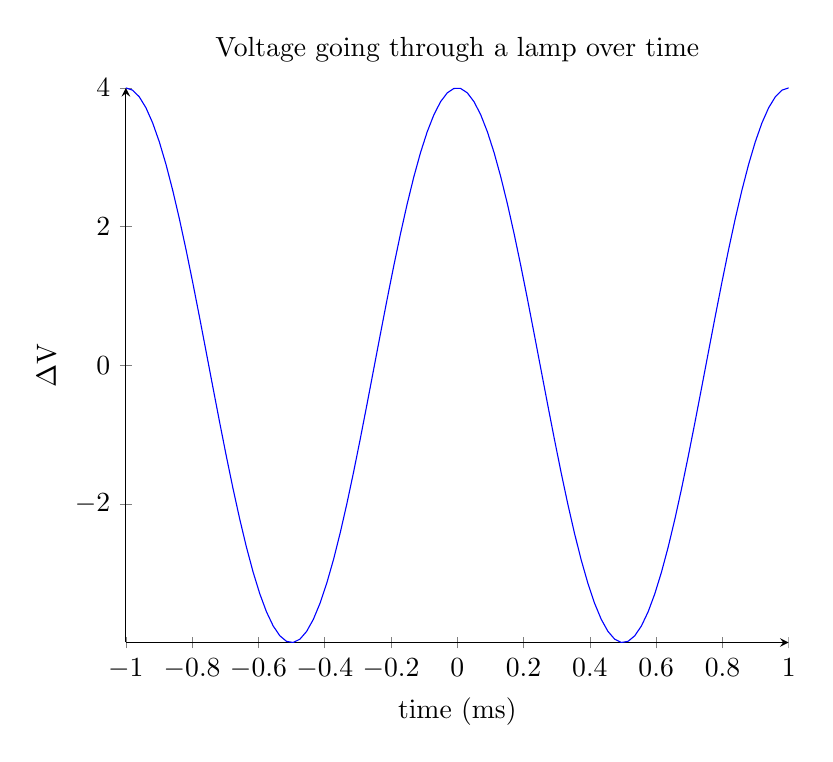
\begin{tikzpicture}
    \begin{axis}[
        axis lines = left,
        title = Voltage going through a lamp over time,
        xlabel = time ($\si{\milli\second}$),
        ylabel = $\Delta\si{\volt}$,
        ]        
        \addplot[
            domain=-1:1,
            samples=100,
            color=blue,
            ]
            {sin(deg((x+0.25)*2*pi))*4};
    \end{axis}
\end{tikzpicture}
\begin{gather}
    \Delta\si{\volt}_{\max}=(4.0\pm0.2)\si{\volt}\\
    \Delta\si{\volt}_{rms}=(2.79\pm0.06)\si{\volt} \label{eq:vrmsmeasured}\\
    I_{rms}=(4.0\pm0.2)\si{\volt}\\ 
    T=(1.00\pm0.04)\si{\milli\second}
\end{gather}

\section{Calculations}
\begin{align}
    \Delta\si{\volt}_{rms}&=\frac{\Delta\si{\volt}_{\max}}{\sqrt{2}} \nonumber\\
    \Delta\si{\volt}_{rms}&=\frac{(4.0\pm0.2)\si{\volt}}{\sqrt{2}}\nonumber\\
    \Delta\si{\volt}_{rms}&=(2.8\pm0.1)\si{\volt} \label{eq:vrmscalc}
\end{align}
\begin{align}
    P_{avg}&=\Delta\si{\volt}_{rms}I_{rms}\nonumber\\
    P_{avg}&=(2.79\pm0.06)\si{\volt} * (4.0\pm0.2)\si{\volt} \nonumber\\ 
    P_{avg}&=(0.285\pm0.012)\si{\watt}
\end{align}
\begin{align}
    F&=\frac{1}{T} \nonumber\\
    F &=\frac{1}{(0.0010\pm 0.0004) \si{\second} }\nonumber\\ 
    F &=(1000\pm 40)\si{\hertz} \label{eq:frequencycalc}
\end{align}

\section{Discussion}
The voltage$_{rms}$ measured at~\eqref{eq:vrmsmeasured} agrees with the calculated value at~\eqref{eq:vrmscalc}\\
The frequency calculated at~\eqref{eq:frequencycalc} agrees with the given value of 1000 \si{\hertz}\\
When the frequency was set to 100\si{\hertz}, a time scale of 2\si{\milli}\si{\second}/div was needed for proper observation\\
When the frequency was set to 10\si{\hertz}, a time scale of 20\si{\milli}\si{\second}/div was needed for proper observation. The sine wave shown on the oscilloscope also started flashing\\
Since this is an ac circuit, the lamp should flash twice per period. Thus, by setting the frequency to 1 \si{\hertz} should make the lamp light up 20 times over 10 seconds. This was confirmed when tested, and the lamp does flash twice per period because there are two voltage peaks during one period.

\chapter{AC circuit with an inductor}

\section{Procedure}
\begin{itemize}
    \item Replace the lamp by a 10\si{\milli\henry} inductor.
    \item Set the frequnecy of the AC source to 1800 \si{\hertz}
    \item Adjust the horizontal scale of the oscilloscope to see the sinusoidal pattern on the screen.
    \item Measure the value of $\Delta\si{\volt}_{Lrms}$ and I$_{Lrms}$. Use these values to calculate X$_{L}$ (include uncertainties and units on X$_{L}$).
    \item Use the calculated value of X$_{L}$ to caluclate L with its uncertainties.
    \item Verify that the calculated value of L is in agreement with the nominal value of $(10\pm1)\si{\milli\henry}$
    \item Now set frequency of the AC source to 1600 \si{\hertz}. Observe how the reading of both digital multimeters change. Interpret the variatiation 
    \item Turn off the AC source before performing the next step for safety.
\end{itemize}
    

\subsection{Measurements}
With F=1800Mhz
\begin{gather}
    \Delta\si{\volt}_{Lrms}=(2.73\pm0.06)\si{\volt}\\ 
    I_{rms}=(23.8\pm0.8)\si{\milli\ampere}
\end{gather}
With F=1600Mhz
\begin{gather}
    \Delta\si{\volt}_{Lrms}=(2.73\pm0.06)\si{\volt}\\ 
    I_{rms}=(26.4\pm0.8)\si{\milli\ampere}
\end{gather}
\subsection{Calculations}
\begin{align}
    \Delta\si{\volt}_{Lrms}&=X_{L}I_{rms}\nonumber\\
    X_{L}&=\frac{\Delta\si{\volt}_{Lrms}}{I_{rms}}\nonumber\\
    X_{L}&=\frac{(2.73\pm0.06)\si{\volt}}{(23.8\pm0.8)\si{\milli\ampere}}\nonumber\\
    X_{L}&=(11.47\pm 0.29)\frac{\si{\volt}}{\si{\ampere}} \label{eq:xlcalc}
\end{align}
\begin{align}
    X_{L}&=\omega L\nonumber\\
    L&=\frac{X_{L}}{\omega}\nonumber\\
    L&=\frac{(114.7\pm 0.3)\frac{\si{\volt}}{\si{\ampere}}}{2\pi1800\si{\hertz}} \nonumber\\
    L&=(10.14 \pm 0.26)\si{\milli}\si{\henry}\label{eq:lcalc}
\end{align}
\subsection{Discussion}
The value of L calulated at~\eqref{eq:lcalc} agrees with the nomival value of 10$\si{\milli}\si{\henry}\pm1\si{\milli}\si{\henry}$\\
When the frequency of the ac source was changed to 1600hz the $\Delta\si{\volt}_{Lrms}$ did not change and the I$_{rms}$ went down linearly.

\chapter{ AC Circuit with a capacitor}

\section{Procedure}

\begin{itemize}
    \item Replace the inductor by a $1.0\si{\micro\farad}$ capacitor and set the frequency of the AC source to $1000\si{\hertz}$
    \item Measure the $\Delta\si{\volt}_{Crms}$ and $I_{Crms}$ using both digital multimeters.
    \item Calculate $X_{C}$ using these measurements (ignore uncertainties).
    \item Use the calculated $X_{C}$ to determine C (ignore uncertainties).
    \item Calculate the percent error on C.
    \item Predit the value of $I_{Crms}$ when the frequency of the power source is $600\si{\hertz}$ 
\end{itemize}

\section{Measurements}

\begin{gather}
    \Delta\si{\volt}_{Crms}=2.76\si{\volt}\\
    I_{Crms}=16.8\si{\milli\ampere}\\
    I_{Crms(600hz)}=10.1\si{\milli\ampere}
\end{gather}

\section{ Calculations}

\begin{align}
    \Delta\si{\volt}_{Crms}&=X_{L}I_{Crms}\nonumber\\
    X_{C}&=\frac{\Delta\si{\volt}_{Crms}}{I_{Crms}}\nonumber\\
    X_{C}&=\frac{2.76\si{\volt}}{16.8\si{\milli\ampere}}\nonumber\\
    X_{C}&=164.3\frac{\si{\volt}}{\si{\ampere}}\label{eq:xccalc}
\end{align}
\begin{align}
    X_{C}&=\frac{1}{\omega C}\nonumber\\
    C&=\frac{1}{\omega X_{C}}\nonumber\\
    C&=\frac{1}{2\pi1000\si{\hertz}*164.3\frac{\si{\volt}}{\si{\ampere}}}\nonumber\\
    C&=0.9687\si{\micro\farad}
\end{align}
\begin{align}
    \%error&=100 * (C_{cal} - 1.00\si{\micro\farad})/1.00\si{\micro\farad}\nonumber\\
    \%error&=100 * (0.9687\si{\micro\farad} - 1.00\si{\micro\farad})/1.00\si{\micro\farad}\nonumber\\
    \%error&=3.13\%
\end{align}
\begin{align}
    \Delta\si{\volt}_{Crms}&=X_{L}I_{Crms}\nonumber\\
    I_{Crms}&=\frac{\Delta\si{\volt}_{Crms}}{X_{L}}\nonumber\\
    I_{Crms}&=\frac{2.76\si{\volt}}{\frac{1}{2\pi*600\si{\hertz}*1.00\si{\micro\farad}}}\nonumber\\
    I_{Crms}&=10.4\si{\milli\ampere}\label{eq:icrmscalc}
\end{align}

\section{Discussion}

I predicted that the current would go down to 10.4\si{\milli\ampere} as calculated in\eqref{eq:icrmscalc}. However, the measured I$_{Crms}$ went down to 10.1mA. A logical explanation for this would be that I wrongly assumed the voltage would stay identical, but since I have control of the source, I dont believe that to be correct. A 3\% difference could've been explained by uncertainties in both the calculation and the measurement.




\end{document}
